\section{Implementation of an OpenDT prototype}\label{sec:prototype}
In this section, we present implementation details of OpenDT, matching step 5 from the community-standard research methodology on the distributed systems. In this early prototype, due to time resource constrains, we couple OpenDT with data obtained from a real-world datacenter and used in peer-reviewed literature; we planned future work in coupling OpenDT with real-world ICT infrastructure, which would send telemetry data to the OpenDT and receive adjustment feedback from OpenDT.


\subsection{Dataset}\label{sec:dataset}

To replicate the real-world infrastructure (i.e., physical twin), we replay data from the FAIR dataset of SURF-22, a scientific workload trace used in peer-reviewed experiments~\cite{DBLP:conf/wosp/NiewenhuisTIM24, nicolae5377101m3sa}. SURF-22 was traced in one of the largest HPC facilities at SURF, Netherlands, over 7 days, in October 2022, and contains anonymised scientific jobs run in production, batch, with an average duration of 39.52 CPU-hours and also detailed energy use over the same period~\cite{nicolae5377101m3sa}. The SURF workload contains 7,850 tasks, and 2,323,475 corresponding fragments, spanning in total approximately 310,000 CPU hours, and are sampled at a granularity of 30 seconds~\cite{nicolae5377101m3sa}. Many thanks to AtLarge Research and our collaborators from SURF for the FAIR dataset released to open-science.


\begin{table}[t]
\centering
\renewcommand{\arraystretch}{1.1}
\begin{tabularx}{\linewidth}{l l l X}
\toprule
\textbf{Field} & \textbf{Data type} & \textbf{Unit} & \textbf{Description} \\
\midrule
id               & string   & —    & Unique identifier \\
duration         & int64    & ms   & Duration of task \\
submission\_time  & datetime & —    & Time of task submission \\
cpu\_count       & int32    & count& Number of CPUs required \\
cpu\_capacity     & float64  & MHz  & CPU capacity required \\
mem\_capacity     & int64    & MB   & Memory required \\
\bottomrule
\end{tabularx}
\caption{Schema of the tasks dataset. A workload task compatible with OpenDC contains multiple fragments, as detailed in~\cite{opendc-workload}.}
\label{tab:tasks_schema}
\end{table}


\begin{table}[t]
\centering
\renewcommand{\arraystretch}{1.1}
\begin{tabularx}{\linewidth}{l l l X}
\toprule
\textbf{Field} & \textbf{Data type} & \textbf{Unit} & \textbf{Description} \\
\midrule
id            & string  & —    & Unique identifier \\
duration      & int64   & ms   & Duration of fragment \\
cpu\_count     & int32   & count& Number CPUs used in fragment \\
cpu\_capacity  & float64 & MHz  & CPU capacity used in fragment \\
\bottomrule
\end{tabularx}
\caption{Schema of the fragments dataset. OpenDC is compatible with the fragments schema explained in~\cite{opendc-workload}.}
\label{tab:fragments_schema}
\end{table}

\Cref{tab:tasks_schema} presents the schema underlying the tasks component and \Cref{tab:fragments_schema} presents the schema of the fragments component of the SURF-22 dataset. In the SURF-22 workload, OpenDC-compatible, fragments are ordered and grouped into chunks and all the fragments beloning to a task share the same id, specifically the ID of the parent task.

\textit{Performed data processing:} The FAIR dataset of SURF-22 was already compatible with OpenDC, thus we did not conduct any data processing steps. However, in the past, the SURF-22 dataset has been processed by AtLarge Research Group mainly by anonymizing the scientific tasks, ensuring exact compatibility between the data file received from SURF and the input schema needed by OpenDC, and, ultimately, releasing the resulting data file as a FAIR dataset.

We use the SURF-22 dataset as a temporary replacement for the physical twin component. We have planned future work in coupling OpenDT with physical twin, which would provide real-time, real-world telemetry to the digital twinning ecosystem OpenDT underlies. In a real-world setup, similarly, OpenDT would receive telemetry data of both the workload (e.g., which tasks need to be executed, estimated time) and sensor-measured telemetry data (e.g., hardware resource utilization, energy consumption, temperature, cooling).


\subsection{Processing windows} \label{sec:processing_windows}
OpenDT contains a (virtual-) physical twin, underlying Apache Kafka, a state-of-the-art distributed event log and streaming platform, widely used in the community for high-throughput event streaming, and durable event history storage~\cite{kafka, kreps2011kafka}. We configure a replaying granularity of 5 minutes, following the industry standard~\cite{DBLP:conf/ccgrid/MastenbroekAJLB21, DBLP:journals/fgcs/MastenbroekMBI25}, based on the timestamp of the task, and, thus, of the fragment. The starting time of the replay is the smallest timestamp from the workload trace. After every window, the state of the digital twin is multi-layer updated: the simulation component predicts energy consumption and resrouce utilization, the newly arrived tasks are considered, the LLM's suggestions of topology improvement are displayed, awaiting for user's acceptance, etc. 

For demonstrational purposes, we implement a configurable ratio between the replay granularity and the demo-granularity; for example, if the real-world granularity is 300 seconds (i.e., 5 minutes), Kafka streams from SURF-22 pre-defined file, and the ratio is 1:10, the 5 minutes of (virtual-)real-world operation would be executed within 30 seconds. A granularity of 1:100 and 300 seconds of (virtual-)real-world operation would lead to 3 seconds. 

\subsection{Operations done in a processing window}
All the algorithms and analyses are conducted at the window granularity and, thus, an identical process is performed for each window. 
Firstly, OpenDC simulator predicts, for each window, the SLO objectives (e.g., predicts the energy consumption and execution time of the workload in subject). 
Secondly, the OpenDT orchestrator processed the OpenDC's predictions and forwards them to an LLM component (further expanded in~\Cref{sec:design:llm}), which assesses the alignment with the practitioner-established SLOs and, if needed, suggests the practitioner topology adjustments towards fulfilling the SLOs. 
Thirdly, the LLM outputs topology adjustments and displays them to the dashboard, where the human-in-the-loop can approve or reject the changes (we expand the crucial importance of the human-in-the-loop for major decisions in~\Cref{sec:design:choices}).
Lastly, on the approval of the supervising practitioner, the infrastructure is adjusted. 
All data is saved in a datalake, thus aiding for potential investigation, operation, or processing such as historical replay, operational analysis, or incident reports. 



\subsection{Visualization and System Outputs}

The OpenDT platform prototype has a unique control panel that shows the current state of the system, including the datacenter topology and information about current tasks and fragments. The main view \Cref{fig:dashboard} focuses on the details of the current simulation powered by the Digital Twin. This allows operators to analyze the information and take decisions from a single interface, instead of using multiple tools.

\begin{figure}[t]
    \centering
    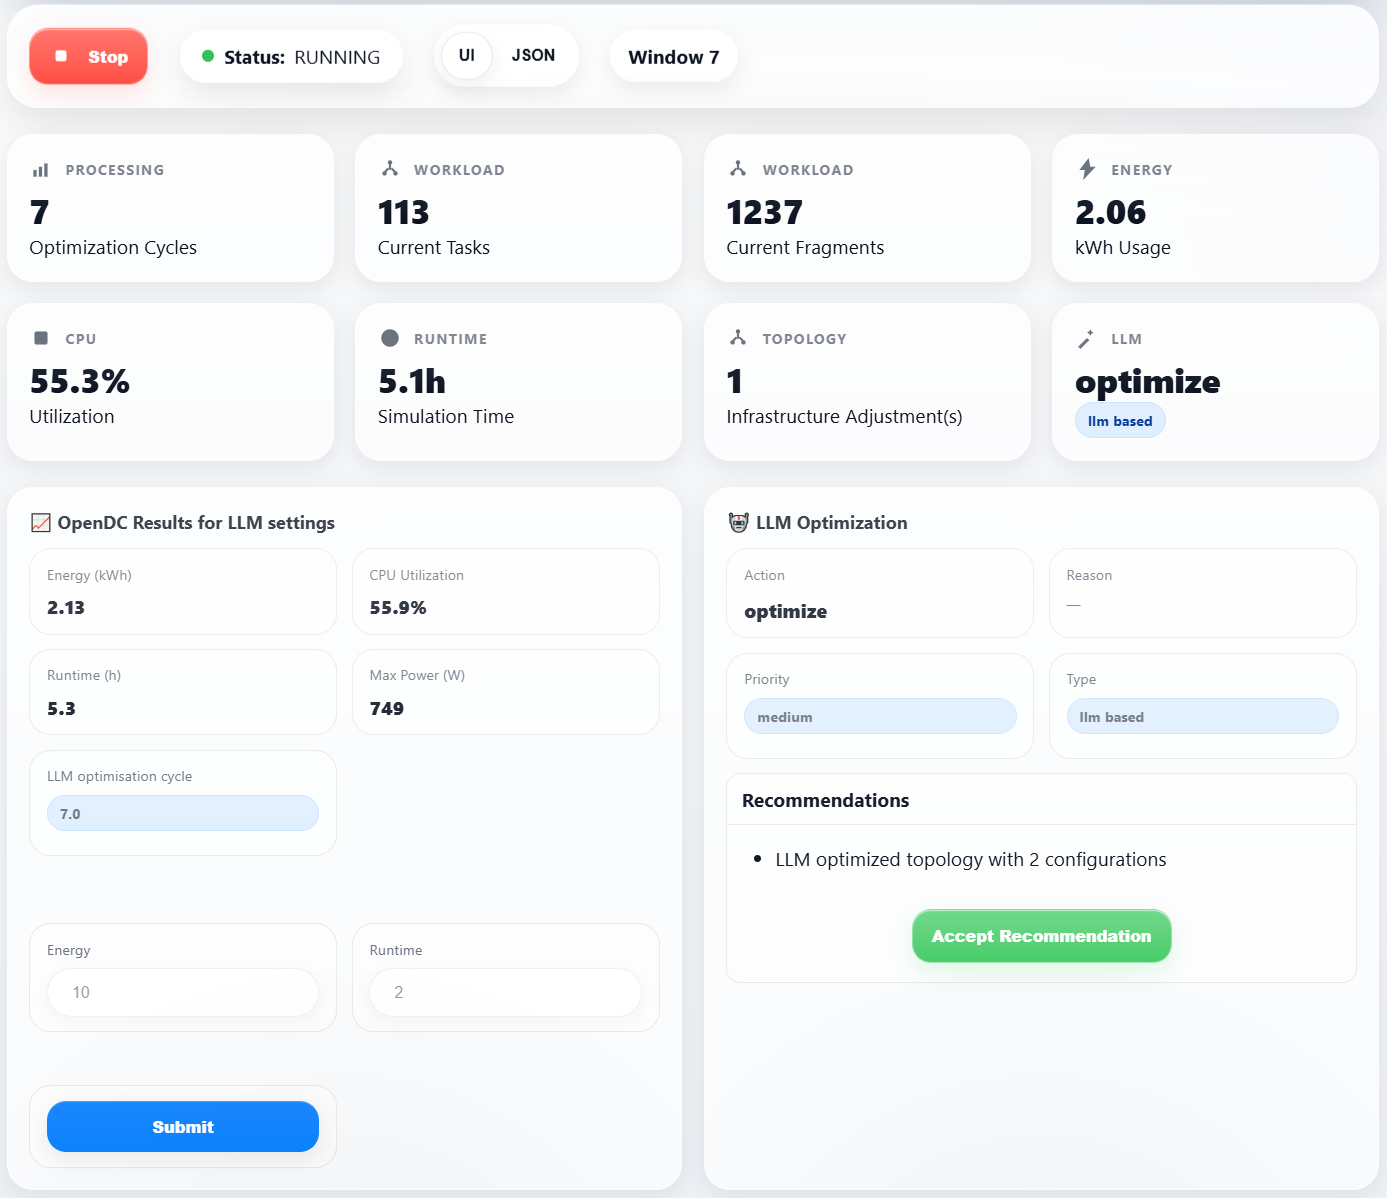
\includegraphics[width=\linewidth]{figures/dashboard.png}
    \caption{OpenDT Digital Twin Dashboard integrating real-time telemetry, simulation results, and LLM-guided topology recommendations.}
    \label{fig:dashboard}
\end{figure}

The panel shows the following useful data: optimization cycles, workload (current task and fragments), energy usage (kWh), CPU utilization, simulation time, and current topology. In addition, an optimization panel can be found. The panel allows the operator to set the energy and runtime in alignment with the SLO's that are then feed into the LLM model for the optimization process.  Afterwards, the operator can accept the recommended topology. The recommendations appear in the same panel, or it can be viewed as a structured JSON record.

Additionally, the visualization has three real-time plots that allow for a direct comparison between the physical and digital twins. \Cref{fig:cpu_plot} shows the evolution of CPU utilization over time. The blue line is the telemetry data obtained from the real datacenter, while the orange dashed line is the result from the OpenDC simulation. The alignment of the two curves can indicate a correct mapping of the workload and allows the operator to identify general use patterns.

\begin{figure}[t]
    \centering
    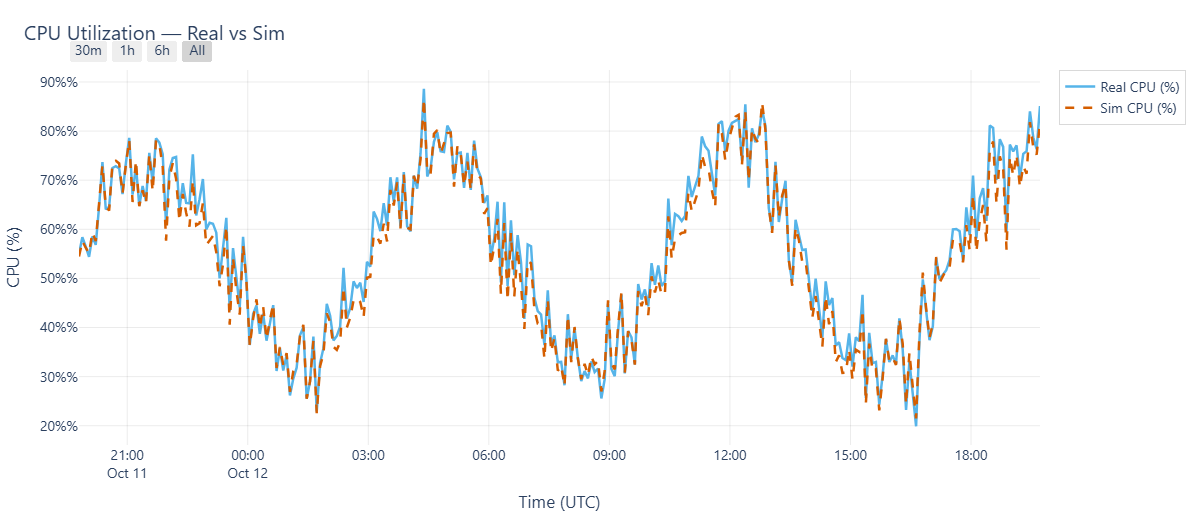
\includegraphics[width=\linewidth]{figures/cpu_plot.png}
    \caption{CPU utilization comparison between real and simulated datacenter telemetry.}
    \label{fig:cpu_plot}
\end{figure}

Similarly, \Cref{fig:power_plot} shows the energy consumption (watts). The main objective of this view is to outline the energetic behavior between twins in the short term. If the lines diverge during a specific window it can be due to heavier or workloads or fails in the hardware of the physical twin (such as cooling problems) that are not yet implemented. Even so, the operator can use this to quickly alert or take action if needed.

\begin{figure}[t]
    \centering
    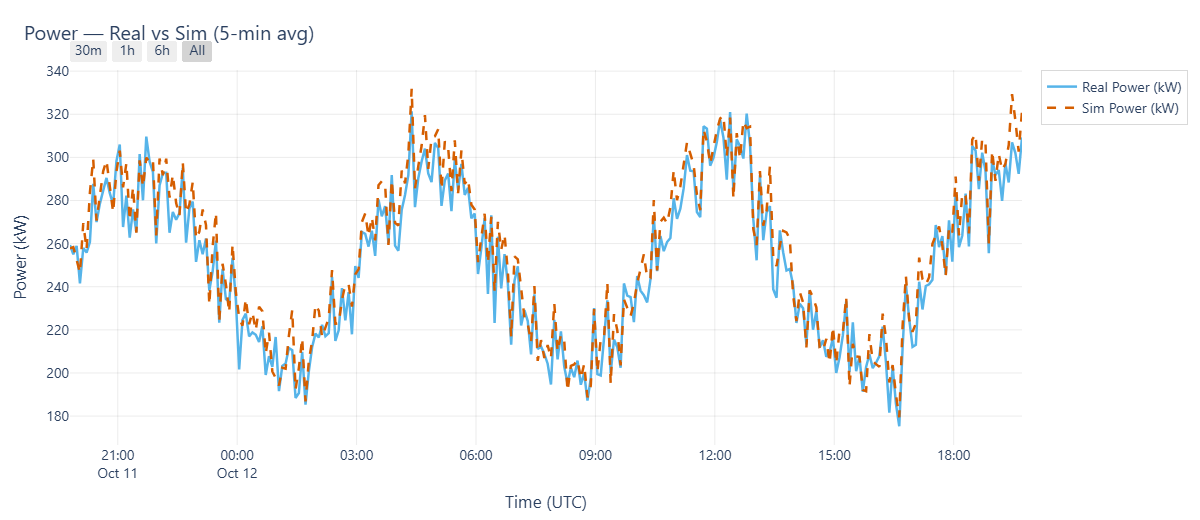
\includegraphics[width=\linewidth]{figures/power_plot.png}
    \caption{Power draw comparison between real and simulated telemetry.}
    \label{fig:power_plot}
\end{figure}

Lastly, ~\Cref{fig:energy_plot} shows the cumulative energy consumption (in kWh) calculated from the power traces. This offers a different point of view focused on the long-term of simulations. A close match between both curves indicates that OpenDT maintains accurate energy estimation across simulations.

\begin{figure}[h]
    \centering
    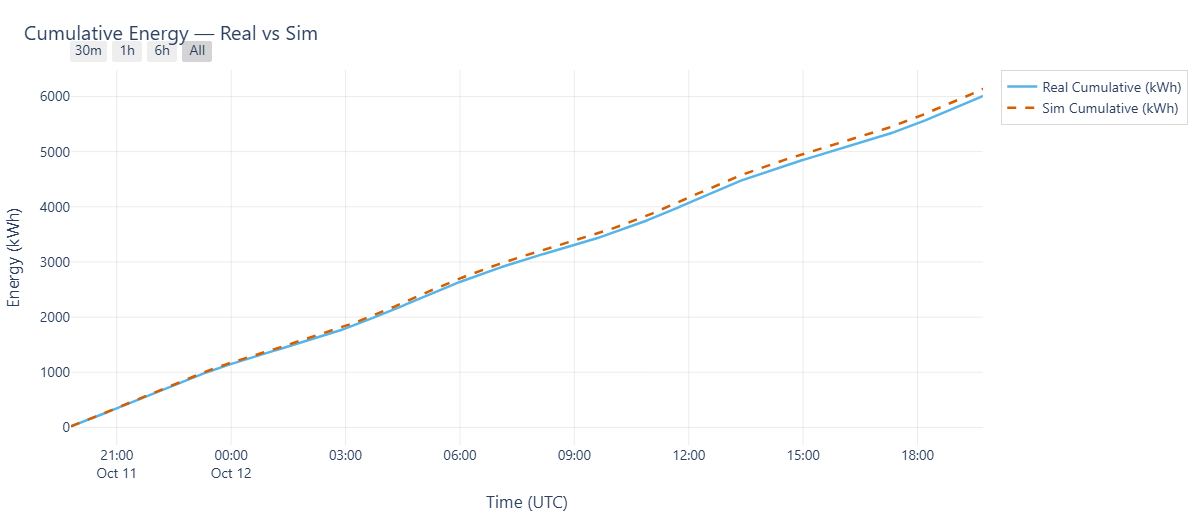
\includegraphics[width=\linewidth]{figures/energy_plot.png}
    \caption{Cumulative energy consumption comparison between physical and digital twins.}
    \label{fig:energy_plot}
\end{figure}

In general, the OpenDT interface transforms the digital twin from a passive simulator into a real-time decision-making tool. By integrating real telemetry and simulation data, with topology recommendations align with clear objectives, allows operators to analyze and verify the fidelity of the digital twin. Furthermore, detecting anomalies and aligning the capacity of the datacenter with SLO's becomes easier and more direct by allowing multiple simulations in a short amount of time. In other words, visualization not only communicates data, but also provides continue feedback between the system and the humans in the loop, making the process interpretable, trustworthy, and actionable in real-world datacenter operation.